
El muestreo aleatorio simple es una de las técnicas más sencillas de tomar una muestra de una población, ya que se basa en la selección de unidades de forma individual y aleatoriamente, según un modelo uniforme discreto, por lo que todos los individuos de la población tienen la misma probabilidad de ser elegidos.\\

En la práctica, para seleccionar las muestras mediante este tipo de muestreo se requiere la existencia de un marco que identifique las unidades de muestreo, que son precisamente los elementos de la población. En España, para las estadísticas oficiales dirigidas a la población, este marco de muestreo se basa principalmente en los datos obtenidos del padrón municipal de habitantes, del cual se pueden extraer tanto individuos como hogares facilitando de esta manera una información sumamente valiosa de cara a diseñar diferentes tipos de muestreo. Para el caso de muestras dirigidas a empresas, el INE utiliza el Directorio Central de Empresas (DIRCE) \cite{DIRCE}, el cual reúne en un sistema de información único a todas las empresas española y a sus unidades locales ubicadas en el territorio nacional. Su objetivo básico es hacer posible la realización de encuestas económicas por muestreo. \\

Existen dos variantes de este tipo de muestreo según las características de sus muestras. El muestreo sin reposición impide la posibilidad de incluir individuos repetidos en la muestra a diferencia del muestreo con reposición, lo que repercute en la estimación de parámetros.\\

Tanto en el muestreo sin reemplazamiento como con reemplazamiento la probabilidad de inclusión en la muestra para todos los individuos de la población es:\\
\begin{equation}\label{eq:1}
    \pi_i = \frac{n}{N}
\end{equation}

donde n es el tamaño de la muestra deseada y N el tamaño poblacional.

\section{Selección de muestras} \label{sect:3.1}
La selección de la muestra sobre la que estudiar la variable de interés debe seguir un procedimiento que asegure la aleatoriedad del proceso. Generalmente se distinguen dos procedimientos con sus posibles aplicaciones en el campo de la informática.\\

El método de la urna se basa en introducir todos los elementos de la población en una urna, convenientemente removida, para sacar uno a uno elementos hasta llegar al tamaño de muestra deseado. Al no poder ver el interior de la urna se supone aleatoriedad.\\

En el muestreo con reposición, tras seleccionar un individuo, éste debe ser devuelto a la urna para permitir que pueda salir elegido de nuevo. En el caso de muestreo sin reposición, cada elemento seleccionado no se devuelve a la urna\\

Para lograr un método de selección similar en un programa informático, se deben enumerar las unidades poblacionales del 1 a N, siendo N el tamaño poblacional. Después utilizando un método aleatorio se obtiene un número aleatorio entre 1 y N, obteniendo el índice del individuo seleccionado. El procedimiento se repite tantas veces como muestras se requieran. En el muestreo sin reposición tras la selección de cada individuo éste se retiraría de la lista y sería necesario tener un control extra sobre el número aleatorio para que no se repita. Un ejemplo sería seleccionar uno nuevo si coincide con el índice de algún individuo seleccionado previamente.\\

El segundo método consiste en usar tablas de números aleatorios, donde se crea una secuencia de números entre 1 y N. Se elige un punto de partida y se seleccionan tantos elementos de forma secuencial como requiera la muestra. Para ello es preciso numerar los individuos al igual que en el método anterior.\\

\begin{center}
    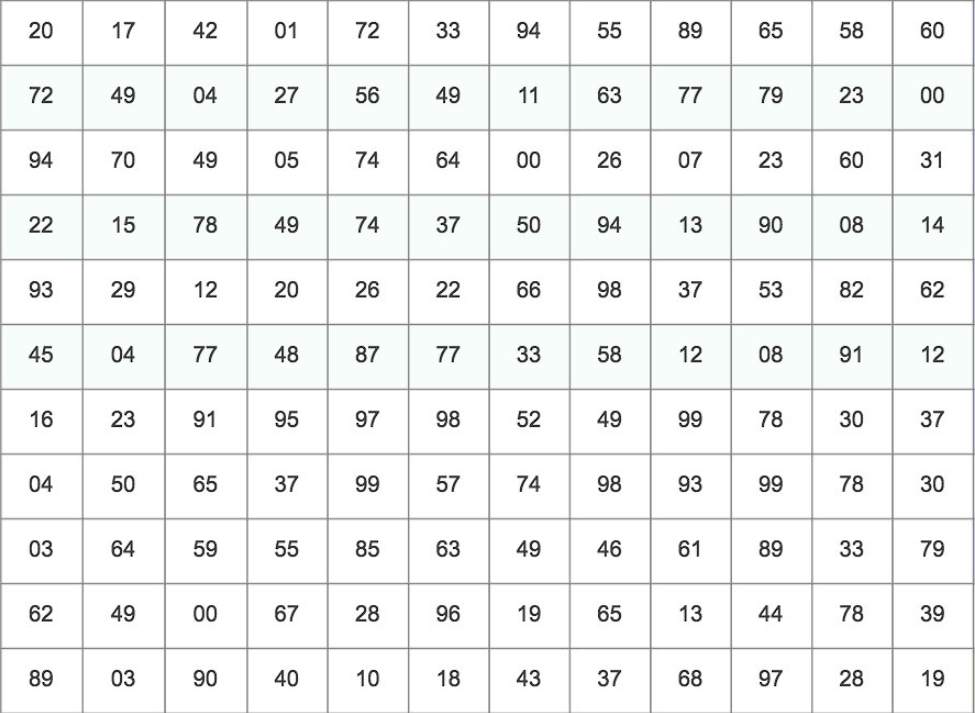
\includegraphics[scale=0.4]{img/tablanumeros.png}
    \captionof{figure}{Ejemplo de tabla de números aleatorios.}
    \label{fig:tablanumeros}
\end{center}

Tomando como ejemplo la figura \ref{fig:tablanumeros} para la selección de una muestra en una población de tamaño 100, se parte desde el primer número, y se seleccionan los números necesarios en orden, bien siguiendo las filas o las columnas, ya que no afecta a la aleatoriedad de la selección. En el caso de querer una muestra de tamaño 5 tomaremos los 5 primeros números de izquierda a derecha o de  arriba hacia abajo, por lo que nuestra muestra constará de los individuos de la población numerados con los índices 20, 17, 42, 1 y 72.\\

Para su aplicación en software informático se indexan los individuos y se utiliza un generador aleatorio de números para obtener tantos números entre 0 y 1 como individuos existen en la población. De entre esos números se seleccionan tantos valores como se requieran para la muestra siguiendo una regla como por ejemplo, utilizando los valores más grandes o los más pequeños, etc. Haciendo coincidir el índice de dichos números con la numeración de la población obtenemos los individuos que forman la muestra aleatoria.\\

En éste trabajo se ha utilizado el método de la urna para la selección de muestras con reemplazamiento y las tablas de números aleatorios para el caso sin reemplazamiento.\\


\section{Estimadores lineales insesgados} \label{sect:3.2}
\subsection{Muestreo aleatorio simple sin reemplazamiento}
Tomando el estimador de Horwitz-Thompson como el estimador lineal insesgado general podemos obtener los estimadores lineales insesgados de los parámetros que precisamos. En concreto, tenemos:\\
\begin{equation}\label{eq:2}
    \hat{\theta}_{HT} = \sum_{i=1}^{n}\frac{Y_i}{\pi_i}
\end{equation}

Para obtener el estimador del total poblacional realizamos el siguiente desarrollo:\\

\begin{equation}\label{eq:3}
    \theta = X = \sum_{i=1}^{N}X_i \Rightarrow Y_i = Xi \Rightarrow \hat{\theta} = \hat{X} = \sum_{i=1}^{n}\frac{X_i}{\pi_i} = \sum_{i=1}^{n}\frac{X_i}{\frac{n}{N}} = N\frac{1}{n}\sum_{i=1}^{n}X_i = N\bar{x}
\end{equation}

Sustituyendo de forma similar para los parámetros media, proporción y total de clase tenemos:\\
\begin{equation}\label{eq:4}
    \hat{\theta} = \hat{\bar{X}} = \sum_{i=1}^{n}\frac{\frac{X_i}{N}}{\pi_i} = \sum_{i=1}^{n}\frac{\frac{X_i}{N}}{\frac{n}{N}} = \frac{1}{n}\sum_{i=1}^{n}X_i = \bar{x}
\end{equation}

\begin{equation}\label{eq:5}
    \hat{\theta} = \hat{P} = \sum_{i=1}^{n}\frac{A_i}{\pi_i} = \sum_{i=1}^{n}\frac{\frac{A_i}{N}}{\frac{n}{N}} = \frac{1}{n}\sum_{i=1}^{n}A_i = P
\end{equation}

\begin{equation}\label{eq:6}
    \hat{\theta} = \hat{A} = \sum_{i=1}^{n}\frac{A_i}{\pi_i} = \sum_{i=1}^{n}\frac{A_i}{\frac{n}{N}} = N\frac{1}{n}\sum_{i=1}^{n}A_i = NP
\end{equation}
Donde $A_i$ son observaciones de una variable dicotómica con valores 0 ó 1.\\

\subsection{Muestreo aleatorio simple con reemplazamiento}
Como ya comentamos al principio de la sección, la probabilidad de inclusión en la muestra para este tipo de muestreo es igual que para el muestreo sin reemplazamiento, por lo que sus estimadores lineales insesgados serán equivalentes a los de las fórmulas \ref{eq:3} a \ref{eq:6}.\\


\section{Estimadores de la varianza} \label{sect:3.3}
\subsection{Muestreo aleatorio simple sin reemplazamiento}

Partiendo de la expresión general del estimador insesgado para el cálculo de la varianza en el muestreo sin reposición:\\

\begin{equation}\label{eq:7}
    \widehat{V(\hat{\theta}_{HH})} = \sum_{i=1}^{n}\frac{Y_i^2}{\pi_i^2}(1-\pi_i) +  \sum_{i<j}^{n}\frac{Y_iY_j}{\pi_i\pi_j}\frac{\pi_{ij}-\pi_i\pi_j}{\pi_{ij}}
\end{equation}

y sustituyendo para los estimadores tenemos: \\

\begin{equation}\label{eq:8}
    \hat{V}(\hat{X}) = N^2(1-f)\frac{\hat{S}^2}{n}
\end{equation}
\begin{equation}\label{eq:9}
    \hat{V}(\hat{\bar{X}}) = (1-f)\frac{\hat{S}^2}{n}
\end{equation}    
\begin{equation}\label{eq:10}
    \hat{V}(\hat{P}) = (1-f)\frac{\hat{P}\hat{Q}}{n-1}
\end{equation}
\begin{equation}\label{eq:11}
    \hat{V}(\hat{A}) = N^2(1-f)\frac{\hat{P}\hat{Q}}{n-1}
\end{equation}

donde $f=\frac{n}{N}$ y la cuasivarianza muestral es un estimador insesgado de la cuasivarianza poblacional, y queda definida por:\\

\begin{equation}\label{eq:12}
    \hat{S}^2 = \frac{1}{n-1}\sum_{i=1}^{n}(X_i-\bar{x})^2
\end{equation}

\subsection{Muestreo aleatorio simple con reemplazamiento} \label{sect:4.3.2}
La expresión general del estimador insesgado de la varianza en el muestreo aleatorio con reemplazamiento es:\\
\begin{equation}\label{eq:13}
    \widehat{V(\hat{\theta}_{HH})} = \frac{1}{n-1}\sum_{i=1}^{n}(\frac{Y_i}{P_i}-\hat{Y}_{HH})^2
\end{equation}

que al aplicarla al estimador del total, media, proporción y total de clase obtenemos:\\

\begin{equation}\label{eq:14}
    \hat{V}(\hat{X}) = N^2\frac{\hat{S}^2}{n}
\end{equation}
\begin{equation}\label{eq:15}
    \hat{V}(\hat{\bar{X}}) = \frac{\hat{S}^2}{n}
\end{equation}    
\begin{equation}\label{eq:16}
    \hat{V}(\hat{P}) = \frac{\hat{P}\hat{Q}}{n-1}
\end{equation}
\begin{equation}\label{eq:17}
    \hat{V}(\hat{A}) = N^2\frac{\hat{P}\hat{Q}}{n-1}
\end{equation}

donde la cuasivarianza muestral $\hat{S}^2$ es un estimador insesgado de la varianza poblacional.\\

Como puede comprobarse estas expresiones son equivalentes a las expresiones \ref{eq:8} a \ref{eq:11} del muestreo sin reposición excepto el factor $(1-f)$.\\
    

\section{Tamaño de la muestra} \label{sect:3.4}
Cuando se realiza el estudio de una variable de interés sobre una población mediante técnicas de muestreo, es deseable que al realizar la estimación se aseguren unas tolerancias en el error.\\

Desarrollando la expresión del error de muestreo e = $\sqrt{ \hat{V}(\hat{\theta})}$ y despejando n se puede obtener el tamaño de muestra que debería tomarse dependiendo del estimador y el tipo de muestreo realizado para lograr los resultados deseados.\\

Las diferentes situaciones que se han usado en este trabajo, son las siguientes:\\

\subsection{Error de muestreo dado}\label{sect:4.4.1}
Es el escenario más simple, en el que determinamos el tamaño de la muestra en base al error de muestreo absoluto a cometer. Tomamos el ejemplo de la estimación para la media en el muestreo aleatorio sin reemplazamiento:\\
\begin{equation}
    e = \sqrt{ \hat{V}(\hat{\theta})} = \sqrt{(1-\frac{n}{N})\frac{S^2}{n}} \Rightarrow n = \frac{NS^2}{Ne^2+S^2} 
\end{equation}

Al tomar muestras con este tamaño es posible que el error de muestreo sea ligeramente mayor que el especificado, pero siempre será cercano a su valor.\\

\subsection{Error de muestreo y coeficiente de confianza dados}\label{sect:4.4.2}
En el caso en el que se desea obtener un error de muestreo menor o igual al especificado de forma más consistente que en el anterior escenario es necesario introducir un coeficiente de confianza $\alpha$ entre 0 y 1 de forma que con probabilidad $1-\alpha$ nos encontremos en la situación deseada.\\

Para ello tomamos $\lambda_\alpha$ como el cuartil de la distribución normal estándar para el valor de $\alpha$ dado. Desarrollando la expresión de la media:\\
\begin{equation}
    e_\alpha = \lambda_\alpha e= \sqrt{(1-\frac{n}{N})\frac{S^2}{n}} \Rightarrow n = \frac{\frac{\lambda_\alpha^2S^2}{e_\alpha^2}}{1+\frac{\frac{\lambda_\alpha^2S^2}{e_\alpha^2}}{N}} = \frac{n_\alpha}{1+\frac{n_\alpha}{N}} 
\end{equation}
Al introducir el coeficiente de confianza el valor de n siempre será mayor que en el apartado \ref{sect:4.4.1}\\

\subsection{Error relativo de muestreo dado}\label{sect:4.4.3}
El error relativo representa otra medida de precisión distinta al error de muestreo y se define como el coeficiente del error de muestreo sobre el parámetro y el valor del parámetro sobre la población, o lo que es lo mismo su valor real.\\
\begin{equation}
    e_r = \frac{ \sqrt{\widehat{V(\bar{X})}} }{E(\bar{X})} = \frac{\sqrt{(1-\frac{n}{N})\frac{S^2}{n}}}{\bar{X}} \Rightarrow n = \frac{N(\frac{S}{\bar{X}})^2}{e_r^2+\frac{(\frac{S}{\bar{X}})^2}{N}} = \frac{NC^2}{e_r^2+\frac{C^2}{N}}
\end{equation}
    
\subsection{Error relativo de muestreo y coeficiente de confianza dados}
Siguiendo la propuesta del apartado \ref{sect:4.4.2} y la expresión del error relativo del apartado \ref{sect:4.4.3} tenemos: \\
\begin{equation}
    e_{r\alpha} = \lambda_\alpha \frac{ \sqrt{\hat{V}(\bar{X})} }{E(\bar{X})} \Rightarrow n = \frac{\lambda_\alpha^2 C^2}{e_{r\alpha}^2 + \lambda_\alpha^2\frac{C^2}{N}}
\end{equation}

Desarrollando para el resto de parámetros y en ambos tipos de muestreo finalmente tenemos:\\
\subsection{Muestreo aleatorio simple sin reemplazamiento}

Se incluye en este apartado un resumen de las fórmulas para estimar los tamaños de muestra en el muestreo irrestricto aleatorio, agrupadas en la tabla \ref{tab:srssamplesize}.\\


\begin{table}[H]
\centering
\begin{tabular}{|c|c|c|c|c|}
\hline
\begin{tabular}[c]{@{}c@{}}Tipo de error\\ Parametro\end{tabular} & Absoluto & Relativo & \begin{tabular}[c]{@{}c@{}}Absoluto y coeficiente \\ de confianza adicional\end{tabular} & \begin{tabular}[c]{@{}c@{}}Relativo y coeficiente\\  de confianza adicional\end{tabular} \\ \hline
Total   &  $\frac{N^2 S^2}{e^2+N S^2}$        &  $\frac{N C^2}{N e_r^2+C^2}$        &  $\frac{\lambda_\alpha^2 N^2 S^2}{e^2+\lambda_\alpha^2 N S^2}$   &            $\frac{\lambda_\alpha^2 N C^2}{N e_{r \alpha}^2+\lambda_\alpha^2 C^2}$               \\ \hline
Media   &   $\frac{N S^2}{N e^2+S^2}$       &    $\frac{N C^2}{N e_r^2+C^2}$      &     $\frac{\lambda_\alpha^2 N S^2}{N e^2+\lambda_\alpha^2 S^2}$    &     $\frac{\lambda_\alpha^2 N C^2}{N e_{r \alpha}^2+\lambda_\alpha^2 C^2}$   \\ \hline
Proporción   &  $\frac{N P Q}{e^2(N-1)+P Q}$        &   $\frac{N Q}{P(N-1) e_r^2+Q}$       &     $\frac{\lambda_\alpha^2 N P Q}{e^2(N-1)+\lambda_\alpha^2 P Q}$  &   $\frac{N Q \lambda_\alpha^2}{e_{r \alpha}^2(N-1) P+\lambda_\alpha^2 Q}$                      \\ \hline
Total de clase  &     $\frac{N^3 P Q}{e^2(N-1)+N^2 P Q}$ &   $\frac{N Q}{P(N-1) e_r^2+Q}$     &         $\frac{\lambda_\alpha^2 N^3 P Q}{e^2(N-1)+\lambda_\alpha^2 N{ }^2 P Q} $ & $\frac{N Q \lambda_\alpha^2}{e_{r \alpha}^2(N-1) P+\lambda_\alpha^2 Q}$  \\ \hline
\end{tabular}
\caption{Tamaños de muestra en el muestreo aleatorio simple sin reemplazamiento.}
\label{tab:srssamplesize}
\end{table}

\subsection{Muestreo aleatorio simple con reemplazamiento}

En la tabla \ref{tab:srssamplesize2} se resumen las fórmulas de estimación del tamaño poblacional en el caso del muestreo aleatorio simple con reemplazamiento.\\


\begin{table}[H]
\centering
\begin{tabular}{|c|c|c|c|c|}
\hline
\begin{tabular}[c]{@{}c@{}}Tipo de error\\ Parametro\end{tabular} & Absoluto & Relativo & \begin{tabular}[c]{@{}c@{}}Absoluto y coeficiente \\ de confianza adicional\end{tabular} & \begin{tabular}[c]{@{}c@{}}Relativo y coeficiente\\  de confianza adicional\end{tabular} \\ \hline
Total  &  $\frac{N^2 \sigma^2}{e^2}$    &  $\frac{C^2}{e_r^2}$  &   $\frac{\lambda_\alpha^2 N^2 \sigma^2}{e^2}$   & $\frac{\lambda_\alpha^2 C^2}{e_{r \alpha}^2}$  \\ \hline
Media      &   $\frac{\sigma^2}{e^2}$    &   $\frac{C^2}{e_r^2}$   &    $\frac{\lambda_\alpha^2 \sigma^2}{e^2}$    & $\frac{\lambda_\alpha^2 C^2}{e_{r \alpha}^2}$     \\ \hline
Proporción     &   $\frac{P Q}{e^2}$       &   $\frac{Q}{P e_r^2}$       &   $\frac{\lambda_\alpha^2 P Q}{e^2}$        &     $\frac{\lambda_\alpha^2 Q}{P e_{r \alpha}^2}$                 \\ \hline
Total de clase        &   $\frac{N^2 P Q}{e^2}$       &   $\frac{Q}{P e_r^2}$       &     $\frac{N^2 \lambda_\alpha^2 P Q}{e^2}$            &          $\frac{\lambda_\alpha^2 Q}{P e_{r \alpha}^2}$            \\ \hline
\end{tabular}
\caption{Tamaños de muestra en el muestreo aleatorio simple con reemplazamiento.}
\label{tab:srssamplesize2}
\end{table}


\section{Dominios de estudio} \label{sect:3.5}
Es posible que dentro de la población los individuos estén divididos en subpoblaciones o dominios de los cuales interesa estudiar la variable de interés sobre una de ellas. El problema reside en que no siempre el marco de estudio permite muestrear la subpoblación deseada hasta que no se evalúan los individuos de un marco más general. \\

Una vez tomada una muestra y etiquetados sus individuos en dominios, es posible estudiar la variable de interés para dicho dominio. Para el caso de la media de un dominio tendríamos:
\begin{equation}
    \hat{\bar{Y_j}} = \sum_{k=1}^{n_j}Y_{jk}
\end{equation}
Donde $Y_{jk}, k=1...n_j$ son las medidas de la variable de interés para cada individuo del dominio y $n_j$ el tamaño del dominio dentro de la muestra.\\

Para la estimación de la varianza usaríamos 
\begin{equation}
    \widehat{V(\hat{\bar{Y_j}})} = (1-\frac{n_j}{N_j})\frac{\hat{S_j^2}}{n_j}
\end{equation}
Donde $\hat{S_j^2}$ es la cuasivarianza muestral del dominio y $N_j$ el tamaño del dominio en la población. En caso de no conocer éste último parámetro se puede realizar la aproximación $\frac{n_j}{N_j} = \frac{n}{N}$. \\

\section{Aplicaciones en la librería samplingR}

Las funciones desarrolladas para la aplicación de los conceptos teóricos mostrados anteriormente utilizarán el prefijo \textit{srs} como abreviación de \textit{simple random sampling}, y son las siguientes.

\begin{itemize}[label=$\bullet$]
    \item srs.sample: Dado un tamaño poblacional N y un tamaño de muestra n devuelve una muestra aleatoria simple. Dicha muestra puede ser tomada con o sin reemplazamiento, dependiendo del valor del parámetro \textit{replace}. En caso de aportar un conjunto de datos devolverá los individuos de los datos que conforman la muestra. Al ser esto opcional, si no se aporta un conjunto de datos devolverá los índices de los individuos que conforman la muestra.\\

    Realiza las funciones explicadas en el apartado \ref{sect:3.1}.

    \item srs.estimator: Dada una muestra de datos obtiene el estimador poblacional del parámetro especificado, entre \textit{total poblacional}, \textit{media}, \textit{proporción} y \textit{total de clase}. También calcula su varianza estimada, error de muestreo y opcionalmente su error de estimación y un intervalo de confianza si se especifica el coeficiente de confianza en el parámetro \textit{alpha}. \\

    Se permite especificar si el muestreo se realiza con o sin reemplazamiento para realizar estimaciones más precisas.\\

    Realiza las funciones explicadas en el apartado \ref{sect:3.2} y \ref{sect:3.3}.

    \item srs.domainestimator: Realiza las mismas estimaciones de la función anterior, pero sobre una subpoblación o dominio de los datos muestrales.\\

    Realiza las funciones explicadas en el apartado \ref{sect:3.5}.

    \item srs.samplesize: Calcula el tamaño de muestra necesario para cometer un error de muestreo menor del especificado. Dicho error puede ser absoluto o relativo, según el parámetro \textit{relative}, y se permite la relajación de su estimación si se especifica un coeficiente de confianza. \\

    Para la estimación no se pide aportar los datos poblacionales por la posibilidad de no disponer de ellos, si no que se deben aportar medidas estadísticas tales como la estimación de la varianza y el tamaño poblacional. También se puede especificar el tipo de muestreo que se va a utilizar para realizar estimaciones más precisas.\\

    Aplica los conceptos explicados en el apartado \ref{sect:3.4}.


\end{itemize}
